\documentclass[multi,preview,varwidth=false,border=5,12pt]{standalone}
%\documentclass[12pt]{article}

\newcounter{Qnum}
\usepackage{assignments}
\standaloneenv{question}


%\excludecomment{solution}\let\endsolution\relax


\begin{document}

\begin{center}
\section*{Flow of fluids}
\end{center}

\begin{question}

A tank contains 8733 lbs of water at room temperature. How many hours would it take to empty the tank if a pump removes 2.5 gallons of water from the tank every minute.

\begin{solution}

First, let's figure out how many gallons of water we have.

\begin{align*}
    V=\frac{w}{\gamma}=\frac{8733~\lb}{62.21~\lb/\ft^3}=140.4~\ft^3\times\left(\frac{7.48~\gal}{\ft^3}\right)=1050~\gal
\end{align*}

If we remove 2.5 gallons of water every minute it would take

\begin{align*}
    \left(1050~\gal\right)/(2.5~\gal/\min) = 420 ~\min \times \left(\frac{1~\hr}{60~\min}\right)=7~\hr
\end{align*}

\end{solution}

\end{question}


\begin{question}

If 400 L/min of fluid flows through a DN 50 Schedule 80 steel pipe what is the resulting average velocity (in m/s) of flow?

\begin{solution}
\begin{align*}
A_{\rm flow}=1905~\mm^2=1.905\times 10^{-3}~\m^2\\
Q=400~\mathrm{L}/\min \times \frac{1~\m^3/s}{60,000~\mathrm{L}/\min} = 6.67\times 10^{-3}~\m^3/s\\
\\
v=\frac{Q}{A_{\rm flow}}=\frac{6.67\times 10^{-3}~\m^3/s}{1.905\times 10^{-3} ~\m^2}=3.5~\m/s
\end{align*}
\end{solution}

\end{question}


\begin{question}

What is the smallest size standard Schedule 40 steel pipe that would carry 2.80 L/min of oil with a an average flow velocity below 0.3 m/s?  Report your answer as a metric Nominal Pipe Size (DN).

\begin{solution}
First find the area required to transport the fluid exactly as specified.

\begin{align*}
Q=2.80~\mathrm{L}/\min \times \frac{1~\m^3/s}{60,000~\mathrm{L}/\min} = 4.67\times 10^{-5}~\m^3/s\\
\\
A=\frac{Q}{v}=\frac{4.67\times 10^{-5}~\m^3/s}{0.3~\m/s}=1.56\times 10^{-4}~\m^2=155.56~\mm^2
\end{align*}

If we made the area any smaller the flow velocity would go above the 0.3 m/s.
We therefore must go with DN15 pipe which has an area of 196 mm$^2$.  If we went with the DN10 the flow velocity would be 0.38 m/s.  Going with the DN15 results in a flow velocity of 0.24 m/s.

\end{solution}

\end{question}



\begin{question}

An aneurysm is an abnormal enlargement of a blood vessel such as the aorta.  A  patient's abdominal CT scan reveals an abnormal abdominal aortic diameter of $5.0~\cm$ compared to their normal aortic diameter of $2.5~\cm$.  If blood of density $1060~\kg/\m^3$ travels through the normal portion of the aorta at a speed of $40~\cm/s$ by how much does the pressure in the abnormal region exceed that of the normal region?  Report your answer in kPa.

\begin{solution}
\begin{align*}
\Delta p = \frac{\rho}{2}\left(v_1^2-v_2^2\right)=\frac{\rho v_1^2}{2}\left(1-\left(\frac{d_1}{d_2}\right)^4\right)\\
\Delta p = 0.5\left(1060~\kg/\m^3\right)\left(0.40~\m/s\right)^2\left(1-0.0625\right)=79.5~\Pa
\end{align*}
\end{solution}

\end{question}



\begin{question}

Turpentine is flowing at $0.45~\m^3/s$ in the fabricated tube shown below.  If the pressure before the enlargement at A is 500 kPa what is the pressure at point B?

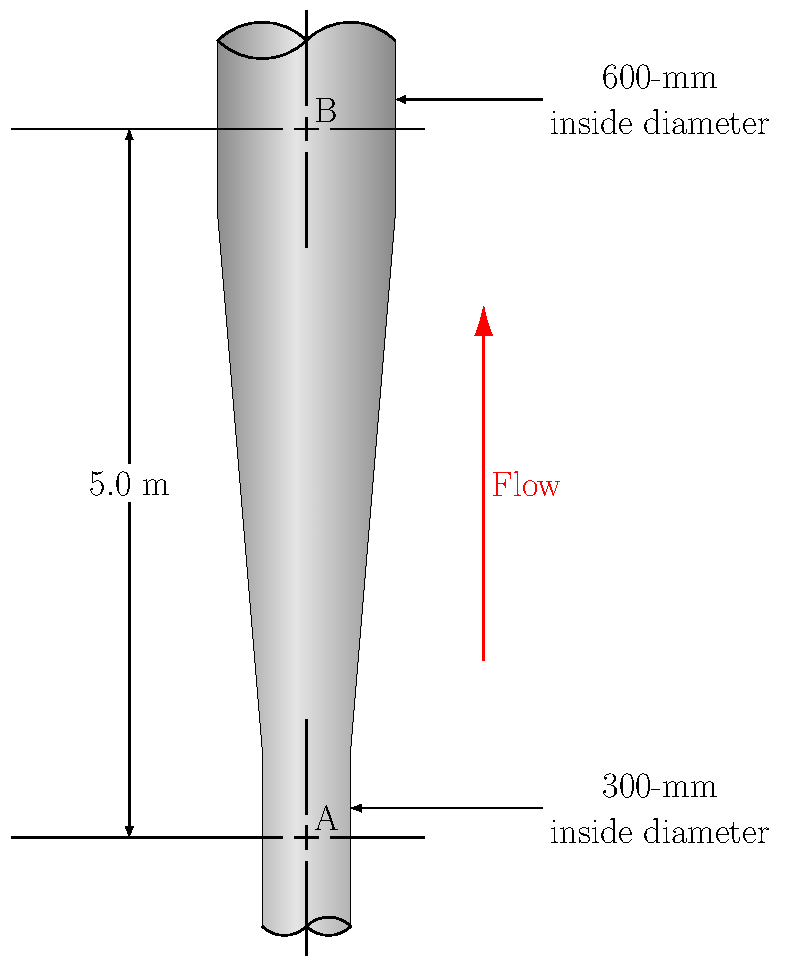
\includegraphics[width=3in]{imgs/PipeExp1.pdf}


\begin{solution}
\begin{align*}
p_B=p_A+\frac{\rho}{2}\left(v_A^2-v_B^2\right)-\gamma (z_B-z_A)\\
v_A=6.37~\m/s\qquad v_B=1.59~\m/s\\
p_B=500~\kPa+\frac{870}{2}\left(6.37^2-1.59^2\right)-8.53 (5~\m)\\
p_B=500~\kPa+16.55~\kPa-42.64~\kPa=474~\kPa
\end{align*}
\end{solution}

\end{question}


\begin{question}

Octane is flowing at 10 gpm from a standard 1-in Schedule 40 steel pipe to a standard 2-in Schedule 40 steel pipe.  The pipes are horizontal.  What is the difference in pressure (in psi) between the two pipes?

\begin{solution}
\begin{align*}
v_{1~\inch}=10~\gpm \frac{1~\ft^3/s}{449~\gpm}\frac{1}{0.006002~\ft^2}=3.71~\ft/s\\
v_{2~\inch}=10~\gpm \frac{1~\ft^3/s}{449~\gpm}\frac{1}{0.02330~\ft^2}=0.956~\ft/s\\
\Delta p = \frac{\rho}{2}\left(v_1^2-v_2^2\right)\\
\Delta p = 0.5\times 1.36\times (3.71^2-0.956^2)~\slug/(\ft\cdot s^2)\\
=8.74~\lb/\ft^2=0.06~\psi
\end{align*}
\end{solution}

\end{question}



\end{document}
